\documentclass[11pt,]{article}
\usepackage[left=1in,top=1in,right=1in,bottom=1in]{geometry}
\newcommand*{\authorfont}{\fontfamily{phv}\selectfont}
\usepackage[]{mathpazo}


  \usepackage[T1]{fontenc}
  \usepackage[utf8]{inputenc}



\usepackage{abstract}
\renewcommand{\abstractname}{}    % clear the title
\renewcommand{\absnamepos}{empty} % originally center

\renewenvironment{abstract}
 {{%
    \setlength{\leftmargin}{0mm}
    \setlength{\rightmargin}{\leftmargin}%
  }%
  \relax}
 {\endlist}

\makeatletter
\def\@maketitle{%
  \newpage
%  \null
%  \vskip 2em%
%  \begin{center}%
  \let \footnote \thanks
    {\fontsize{18}{20}\selectfont\raggedright  \setlength{\parindent}{0pt} \@title \par}%
}
%\fi
\makeatother




\setcounter{secnumdepth}{0}


\usepackage{graphicx,grffile}
\makeatletter
\def\maxwidth{\ifdim\Gin@nat@width>\linewidth\linewidth\else\Gin@nat@width\fi}
\def\maxheight{\ifdim\Gin@nat@height>\textheight\textheight\else\Gin@nat@height\fi}
\makeatother
% Scale images if necessary, so that they will not overflow the page
% margins by default, and it is still possible to overwrite the defaults
% using explicit options in \includegraphics[width, height, ...]{}
\setkeys{Gin}{width=\maxwidth,height=\maxheight,keepaspectratio}

\title{ChangeMyView: Can Moral Appeals Facilitate Persuasion?\thanks{\textbf{Current draft version}: February 25, 2018 --- PLEASE DO NOT CITE
OR REDISTRIBUTE WITHOUT PERMISSION.}  }



\author{\Large Patrick W. Kraft\vspace{0.05in} \newline\normalsize\emph{Stony Brook University}  }


\date{}

% sans serif font
%\renewcommand{\familydefault}{\sfdefault}

% Computer Modern Bright font (sans serif)
%\usepackage{cmbright}
%\usepackage[T1]{fontenc}


\usepackage{titlesec}

\titleformat*{\section}{\normalsize\bfseries}
\titleformat*{\subsection}{\normalsize\itshape}
\titleformat*{\subsubsection}{\normalsize\itshape}
\titleformat*{\paragraph}{\normalsize\itshape}
\titleformat*{\subparagraph}{\normalsize\itshape}


\usepackage{natbib}
\bibliographystyle{/home/patrick/Dropbox/Uni/Lit/apsr2006}
\usepackage[strings]{underscore} % protect underscores in most circumstances



\newtheorem{hypothesis}{Hypothesis}
\usepackage{setspace}

\makeatletter
\@ifpackageloaded{hyperref}{}{%
\ifxetex
  \PassOptionsToPackage{hyphens}{url}\usepackage[setpagesize=false, % page size defined by xetex
              unicode=false, % unicode breaks when used with xetex
              xetex]{hyperref}
\else
  \PassOptionsToPackage{hyphens}{url}\usepackage[unicode=true]{hyperref}
\fi
}

\@ifpackageloaded{color}{
    \PassOptionsToPackage{usenames,dvipsnames}{color}
}{%
    \usepackage[usenames,dvipsnames]{color}
}
\makeatother
\hypersetup{breaklinks=true,
            bookmarks=true,
            pdfauthor={Patrick W. Kraft (Stony Brook University)},
             pdfkeywords = {Moral Foundations, Attitude Change, Persuasion, Political Agreement},  
            pdftitle={ChangeMyView: Can Moral Appeals Facilitate Persuasion?},
            colorlinks=true,
            citecolor=blue,
            urlcolor=blue,
            linkcolor=magenta,
            pdfborder={0 0 0}}
\urlstyle{same}  % don't use monospace font for urls

% set default figure placement to htbp
\makeatletter
\def\fps@figure{htbp}
\makeatother



% add tightlist ----------
\providecommand{\tightlist}{%
\setlength{\itemsep}{0pt}\setlength{\parskip}{0pt}}

\begin{document}
	
% \pagenumbering{arabic}% resets `page` counter to 1 
%
% \maketitle

{% \usefont{T1}{pnc}{m}{n}
\setlength{\parindent}{0pt}
\thispagestyle{plain}
{\fontsize{18}{20}\selectfont\raggedright 
\maketitle  % title \par  

}

{
   \vskip 13.5pt\relax \normalsize\fontsize{11}{12} 
\textbf{\authorfont Patrick W. Kraft} \hskip 15pt \emph{\small Stony Brook University}   

}

}








\begin{abstract}

    \hbox{\vrule height .2pt width 39.14pc}

    \vskip 8.5pt % \small 

\noindent The American electorate is becoming increasingly polarized. Research in
moral psychology suggests that growing disagreements between liberals
and conservatives can be attributed to the fact that they emphasize
different basic moral dimensions. Indeed, scholars suggest that
agreement between ideologues would be easier if both sides spoke the
same \emph{moral language}. However, no study to date tested this
fundamental assumption. Drawing on data from the online discussion board
\emph{Reddit}, this paper examines how varying moral appeals affect
persuasion and the potential for consensus building in politics


\vskip 8.5pt \noindent \emph{Keywords}: Moral Foundations, Attitude Change, Persuasion, Political Agreement \par

    \hbox{\vrule height .2pt width 39.14pc}



\end{abstract}


\vskip 6.5pt


\noindent \doublespacing \section{Introduction}\label{introduction}

Over the recent years, there has been a resurgence in partisan
polarization in the United States. Politically engaged citizens hold
more diverging policy views, are more ideologically extreme, and show
increased affective polarization between partisans
\citep{hetherington2001resurgent, abramowitz2008polarization, iyengar2012affect, mason2014disrespectfully, huddy2015expressive, iyengar2015fear}.
Political discussions among individuals holding diverging views can
mitigate the polarizing effects of partisan motivated reasoning
\citep[see also][]{mendelberg2002deliberative, eveland2011beyond}. In
general, diverse social networks have been shown to reduce attitude
extremity \citep{levitan2009social} and enhance the understanding of
opposing viewpoints \citep{mutz2002cross}. Deliberation in particular
increases political sophistication \citep{gastil1999increasing} and
shapes attitude change towards a common consensus
\citep{vinokur1978depolarization, barabas2004deliberation}.

\citet{druckman2003framing} directly investigated how discussions can
moderate elite framing effects. More specifically, the study focused on
emphasis framing effects, which occur if the information received by an
individual emphasizes a subset of relevant considerations, which in turn
leads individuals to focus on these considerations when forming their
attitude \citep[c.f.][]{druckman2001implications}. In their experiment,
participants were asked to read an article about campaign finance reform
which either focused on the issue of free speech, or special interests.
Subsequently, participants were asked to discuss the issue in small
groups. \citet{druckman2003framing} randomly assigned participants to
groups where all individuals were exposed to the same framing of the
issue (homogeneous condition), or different ones (heterogeneous
condition). Their results showed that discussions in homogeneous groups
had a polarizing effect, whereas discussions in heterogeneous groups had
a depolarizing effect \citep[see also][]{druckman2004political}. As
such, deliberation in diverse groups can decrease the effect of
polarizing elite communication. Similar research was conducted by
\citet{klar2014partisanship}\}, who manipulated group compositions in
terms of the participants' party affiliations rather than comparing
heterogeneous and homogeneous framing conditions. Her results showed
that homogeneous group discussions resulted in more intense partisan
motivated reasoning: individuals reported stronger preferences for the
policies of their in-party and perceived them to be more effective
compared to policies of their out-party. On the other hand, preferences
were less extreme if the social setting was ideologically heterogeneous.

Morality could be viewed as such a potential moderator of deliberation
effects. Whether individuals perceive issues in terms of their
fundamental moral principles can be expected to influence the nature and
tone of political discussions and therefore to moderate the downstream
effects of deliberation in homogeneous and heterogeneous groups.
Consider two scenarios where individuals with opposing attitudes discuss
their views on abortion as compared to the appropriate tax rate. While
both scenarios could result in fierce debates, we can presume that a
group of pro-life and pro-choice advocates will have a harder time to
find a common ground than a group of tax critics and proponents. One
might argue that this difference is simply due to the nature of the
issues themselves. However, how could we then explain potential
differences in willingness to compromise between groups discussing the
same issue? \citet{skitka2005moral} provided a possible answer to this
question by introducing the concept of \emph{moral conviction}\} (or
\emph{moral mandates}) as unique features of attitude strength. In their
view, moral conviction should be regarded as independent from other
dimensions of attitude strength such as extremity, importance, or
accessibility.

Moral convictions are characterized as attitudes that are perceived as
``absolutes, or universal standards of truth that others should also
share'' \citep[269]{skitka2010psychology}. As such, they combine the
following attributes \citep{skitka2010psychology}: they are viewed by
individuals as applying to everyone (universality), they do not require
an immediate underlying rationale but are rather seen as facts about the
world (objectivity), they can be independent of authority and group
norms (autonomy), they elicit strong emotional reactions, and they have
an inherent motivational quality (motivation/justification).

Building on this work, \citet{ryan2014reconsidering} argued that moral
convictions are not restricted to issues that are traditionally
perceived as ``moral'', such as abortion or same-sex marriage, but can
also include other issues such as economic policies.

The degree of moral conviction may therefore vary between individuals as
well as across issues. \citet{ryan2014reconsidering} further showed that
the propensity to moralize -- i.e.~the tendency to view an issue as a
question of ``right and wrong'' -- is related to political
participation, extreme political attitudes, arousal of negative
emotions, and hostility. In a subsequent study, \citet{ryan2016no}
suggested that moralization as a distinct characteristic of attitude
intensity reorients behavior from maximizing gains to the general
adherence to rules. Across multiple studies, the author showed that this
tendency translates into stronger opposition to compromises about
political issues and decreased support for compromising politicians.
These patterns should also translate into attitudes towards -- and
interactions with -- others who hold opposing views. Indeed, moral
conviction has been shown to be related to stronger preferences for
social distance from (and hostility towards) attitudinally dissimilar
others and lower cooperativeness in groups holding heterogeneous views
\citep{skitka2005moral}.

The literature on moral conviction, however, is only beginning to
elaborate on the political implications as the theories were mainly
applied in psychology and did not explicitly consider the political
context. As such, little is known about when and how individuals form
moral convictions for specific political attitudes. For example, what is
the role rhetoric in raising moral mandates and how does moralization
affect subsequent attitude formation and belief updating? Another
important question that is largely unexplored is how people react
towards others who raise potentially conflicting moral considerations in
social interactions? Overall then, all three literatures can benefit
from an integration of the different perspectives, which is the focus of
the next section.

\section{Description of Dataset}\label{description-of-dataset}

\section{\texorpdfstring{\emph{ToDos}}{ToDos}}\label{todos}

\begin{itemize}
\tightlist
\item
  clean original posts (links etc)!
\item
  adjust confidence intervals to correct for multiple comparisons
\item
  add more comments in functions!
\end{itemize}

\section{Moral Foundations and
Persuadability}\label{moral-foundations-and-persuadability}

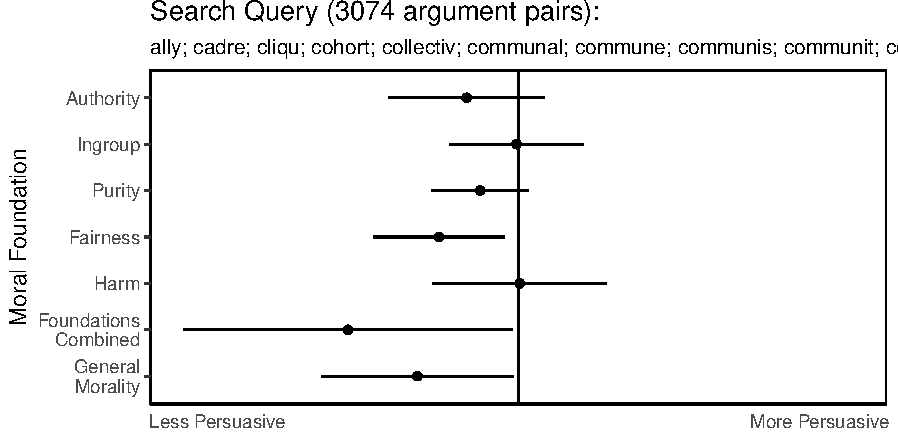
\includegraphics{prelim_files/figure-latex/unnamed-chunk-3-1.pdf}

\section{Is Moral Consistency
Convincing?}\label{is-moral-consistency-convincing}

\emph{Authority}

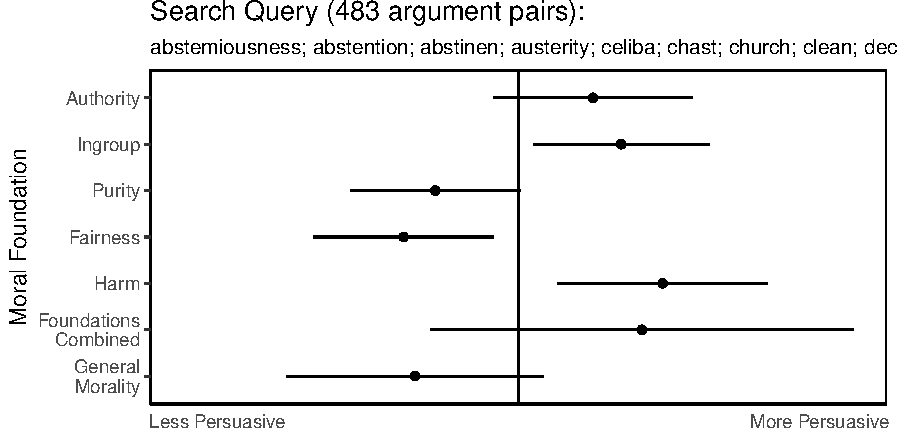
\includegraphics{prelim_files/figure-latex/unnamed-chunk-5-1.pdf}

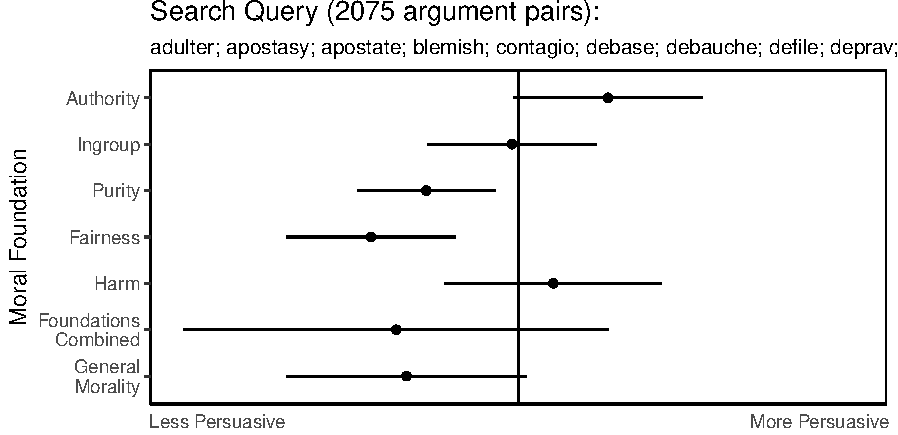
\includegraphics{prelim_files/figure-latex/unnamed-chunk-6-1.pdf}

\emph{Ingroup}

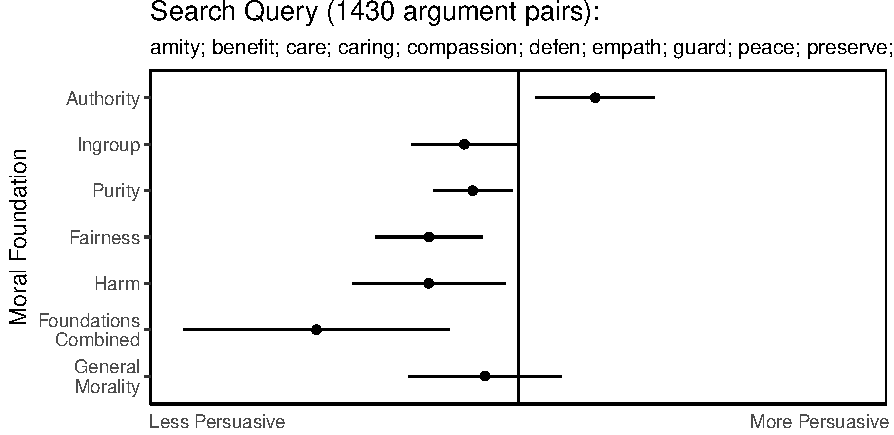
\includegraphics{prelim_files/figure-latex/unnamed-chunk-7-1.pdf}

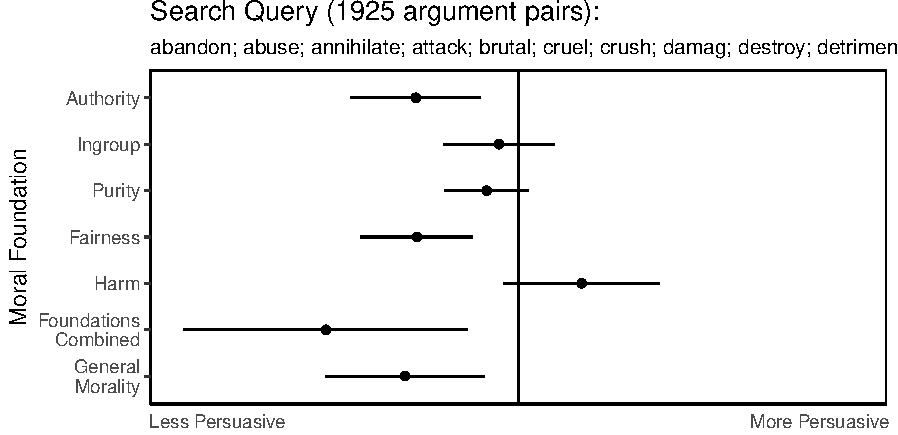
\includegraphics{prelim_files/figure-latex/unnamed-chunk-8-1.pdf}

\emph{Purity}

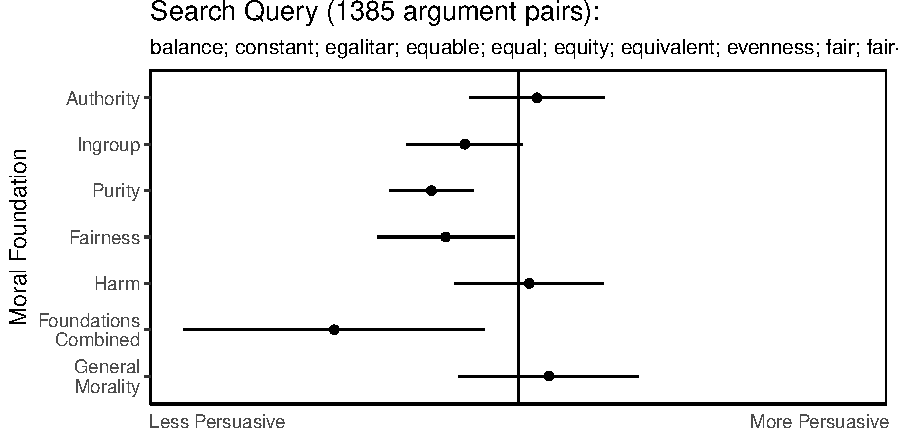
\includegraphics{prelim_files/figure-latex/unnamed-chunk-9-1.pdf}

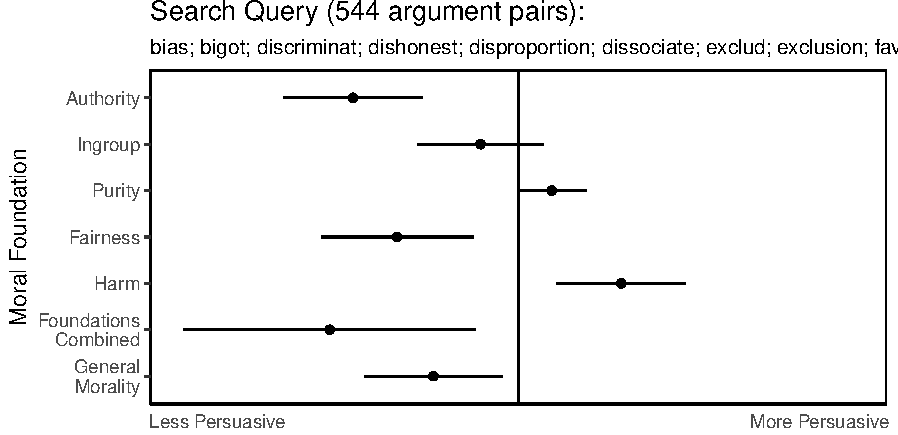
\includegraphics{prelim_files/figure-latex/unnamed-chunk-10-1.pdf}

\emph{Harm}

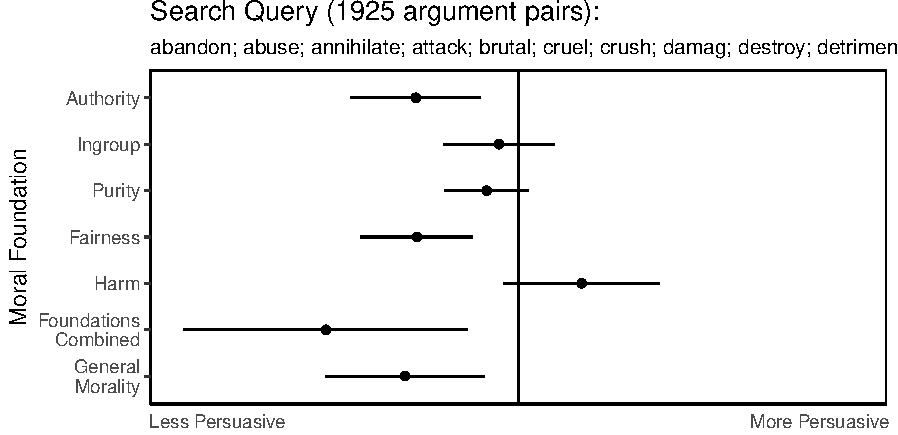
\includegraphics{prelim_files/figure-latex/unnamed-chunk-11-1.pdf}

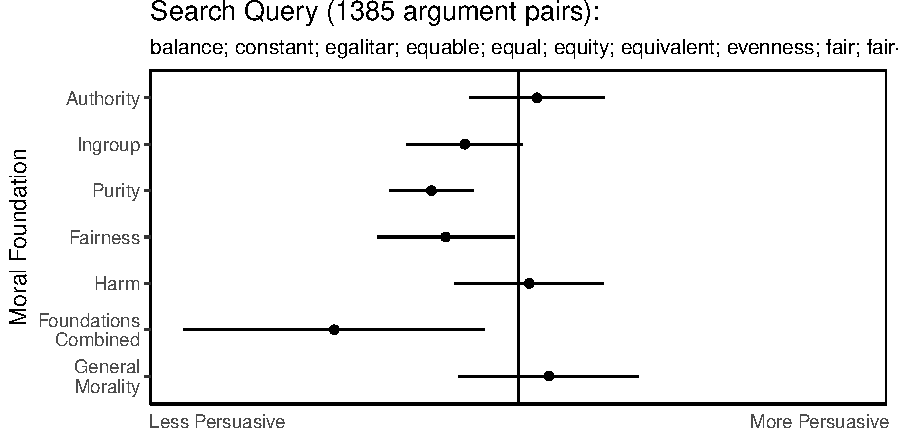
\includegraphics{prelim_files/figure-latex/unnamed-chunk-12-1.pdf}

\emph{Fairness}

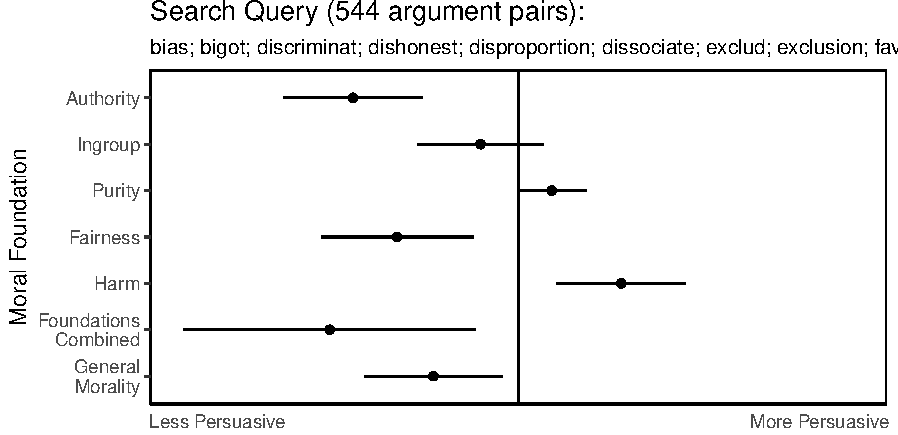
\includegraphics{prelim_files/figure-latex/unnamed-chunk-13-1.pdf}

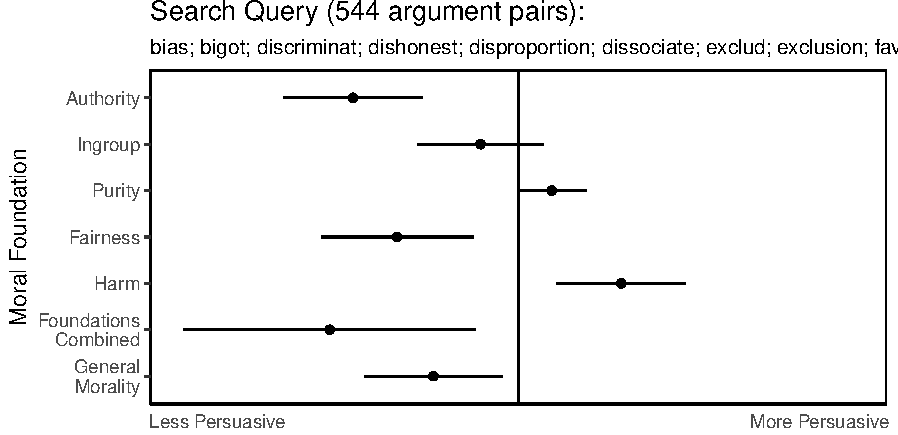
\includegraphics{prelim_files/figure-latex/unnamed-chunk-14-1.pdf}

\section{How about other topics?}\label{how-about-other-topics}

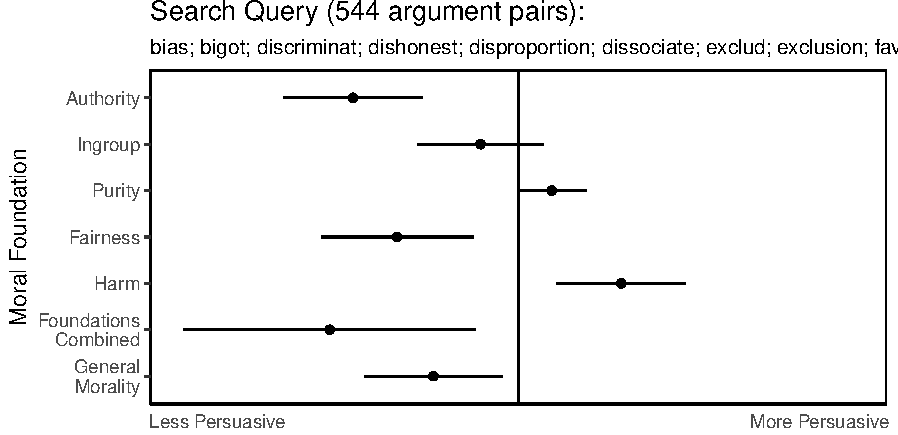
\includegraphics{prelim_files/figure-latex/unnamed-chunk-15-1.pdf}

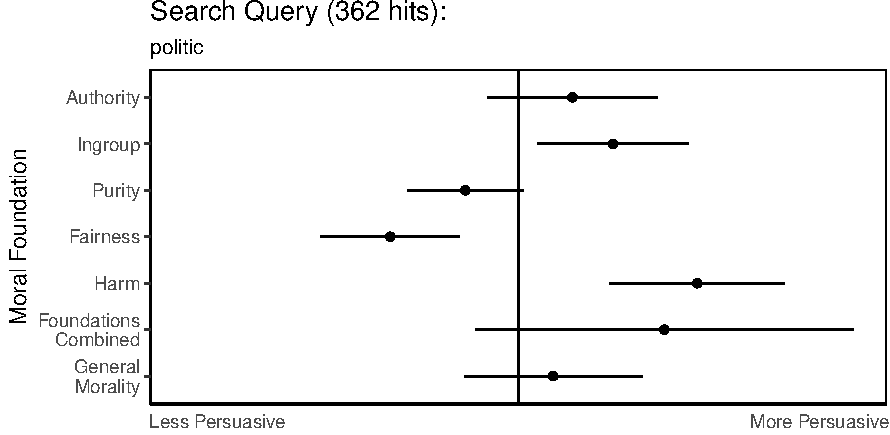
\includegraphics{prelim_files/figure-latex/unnamed-chunk-16-1.pdf}

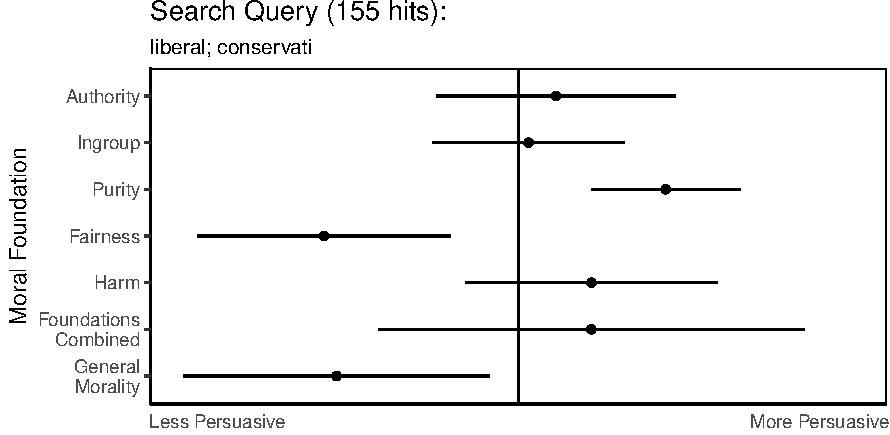
\includegraphics{prelim_files/figure-latex/unnamed-chunk-17-1.pdf}

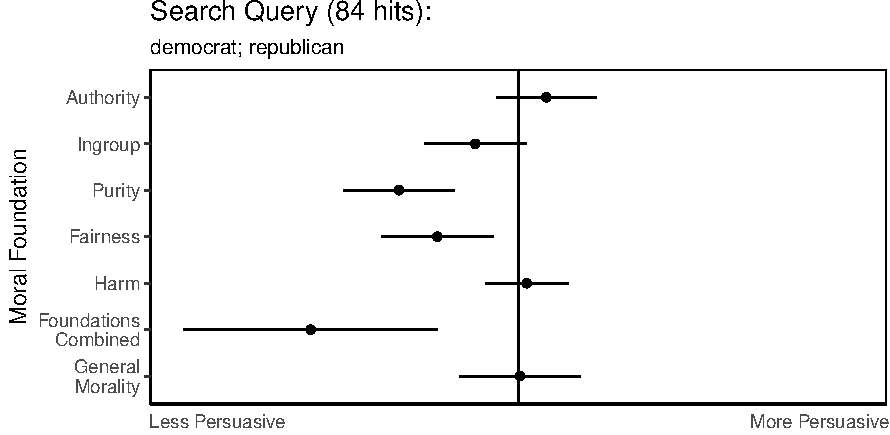
\includegraphics{prelim_files/figure-latex/unnamed-chunk-18-1.pdf}

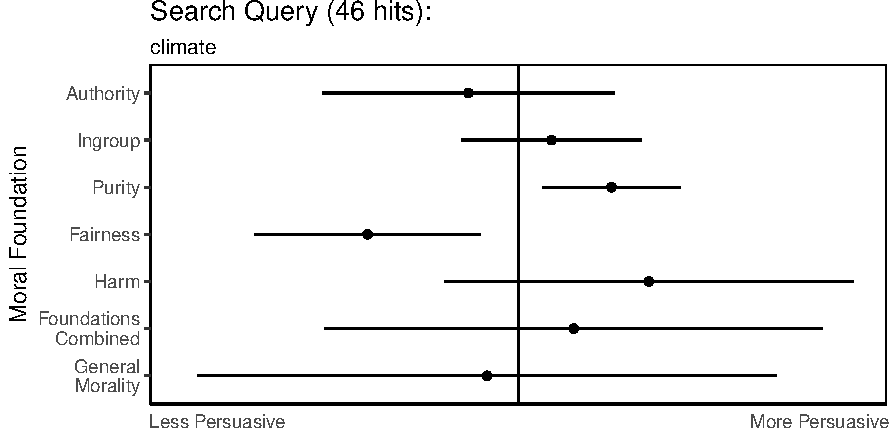
\includegraphics{prelim_files/figure-latex/unnamed-chunk-19-1.pdf}

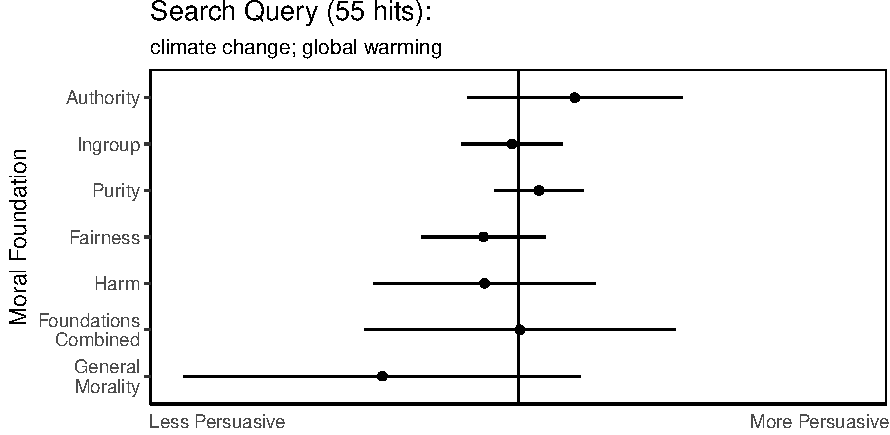
\includegraphics{prelim_files/figure-latex/unnamed-chunk-20-1.pdf}

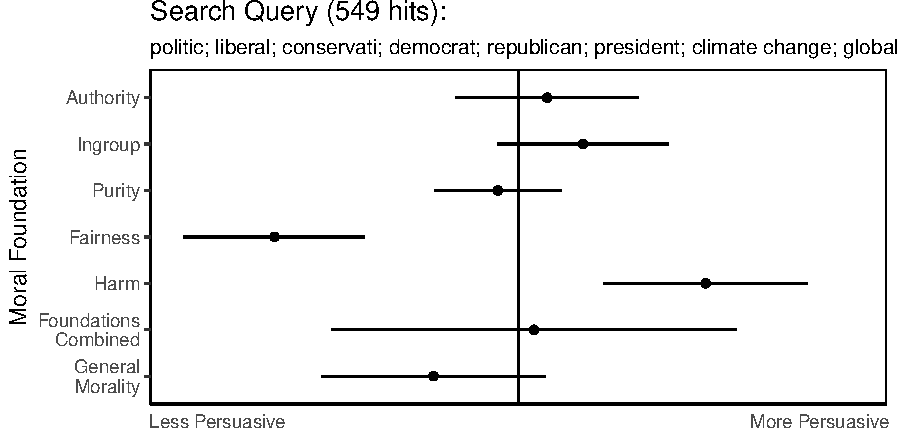
\includegraphics{prelim_files/figure-latex/unnamed-chunk-21-1.pdf}




\newpage
\singlespacing 
\bibliography{/home/patrick/Dropbox/Uni/Lit/Literature}

\end{document}
